%%%%%%%%%%%%%%%%%%%%%%%%%%%%%%%%%%%%%%%%%%%%%%%%%%%%%%%%%%%%%%%%%%%%
%% I, the copyright holder of this work, release this work into the
%% public domain. This applies worldwide. In some countries this may
%% not be legally possible; if so: I grant anyone the right to use
%% this work for any purpose, without any conditions, unless such
%% conditions are required by law.
%%%%%%%%%%%%%%%%%%%%%%%%%%%%%%%%%%%%%%%%%%%%%%%%%%%%%%%%%%%%%%%%%%%%

\documentclass[
  digital,     %% The `digital` option enables the default options for the
               %% digital version of a document. Replace with `printed`
               %% to enable the default options for the printed version
               %% of a document.
%%  color,       %% Uncomment these lines (by removing the %% at the
%%               %% beginning) to use color in the printed version of your
%%               %% document
  oneside,     %% The `oneside` option enables one-sided typesetting,
               %% which is preferred if you are only going to submit a
               %% digital version of your thesis. Replace with `twoside`
               %% for double-sided typesetting if you are planning to
               %% also print your thesis. For double-sided typesetting,
               %% use at least 120 g/m² paper to prevent show-through.
  nosansbold,  %% The `nosansbold` option prevents the use of the
               %% sans-serif type face for bold text. Replace with
               %% `sansbold` to use sans-serif type face for bold text.
  nocolorbold, %% The `nocolorbold` option disables the usage of the
               %% blue color for bold text, instead using black. Replace
               %% with `colorbold` to use blue for bold text.
  lof,         %% The `lof` option prints the List of Figures. Replace
               %% with `nolof` to hide the List of Figures.
  lot,         %% The `lot` option prints the List of Tables. Replace
               %% with `nolot` to hide the List of Tables.
]{fithesis4}
%% The following section sets up the locales used in the thesis.
\usepackage[resetfonts]{cmap} %% We need to load the T2A font encoding
\usepackage[T1,T2A]{fontenc}  %% to use the Cyrillic fonts with Russian texts.
\usepackage[
  main=english, %% By using `czech` or `slovak` as the main locale
                %% instead of `english`, you can typeset the thesis
                %% in either Czech or Slovak, respectively.
  english, german, czech, slovak %% The additional keys allow
]{babel}        %% foreign texts to be typeset as follows:
%%
%%   \begin{otherlanguage}{german}  ... \end{otherlanguage}
%%   \begin{otherlanguage}{czech}   ... \end{otherlanguage}
%%   \begin{otherlanguage}{slovak}  ... \end{otherlanguage}
%%
%%
%% The following section sets up the metadata of the thesis.
\thesissetup{ 
    date        = \the\year/\the\month/\the\day,
    university  = mu,
    faculty     = fi,
    type        = mgr,
    department  = Department of design and development of software systems,
    author      = Bc. Marcel Lukčo,
    gender      = m,
    advisor     = {Mgr. Miroslav Ruda},
    title       = {PBSMon2, web service for displaying MetaCenter status},
    TeXtitle    = {PBSMon2, web service for displaying MetaCenter status},
    keywords    = {cloud, cloud computing, distributed computing, MetaCentrum},
    TeXkeywords = {cloud, cloud computing, distributed computing, MetaCentrum},
    abstract    = {%  
      TBD
    },
    thanks      = {%
    First and foremost, I would like to express my sincere gratitude to my supervisor, Mgr. Miroslav Ruda, for his valuable guidance, insightful comments, and continuous support throughout the development of this thesis.

    I would also like to thank RNDr. Martin Kuba, Ph.D., for his technical assistance and expertise, which significantly contributed to the practical part of this work.
    
    My thanks also go to Mgr. Václav Chlumský, Ing. František Řezníček, and Mgr. Ivana Křenková for their collaboration, helpful advice, and support during the integration with related systems.
    },
    bib         = example.bib,
    %% Remove the following line to use the JVS 2018 faculty logo.
    facultyLogo = fithesis-fi,
}
\usepackage{makeidx}      %% The `makeidx` package contains
\makeindex                %% helper commands for index typesetting.
%% These additional packages are used within the document:
\usepackage{paralist} %% Compact list environments
\usepackage{amsmath}  %% Mathematics
\usepackage{amsthm}
\usepackage{amsfonts}
\usepackage{url}      %% Hyperlinks
\usepackage{markdown} %% Lightweight markup
\usepackage{listings} %% Source code highlighting
\lstset{
  basicstyle      = \ttfamily,
  identifierstyle = \color{black},
  keywordstyle    = \color{blue},
  keywordstyle    = {[2]\color{cyan}},
  keywordstyle    = {[3]\color{olive}},
  stringstyle     = \color{teal},
  commentstyle    = \itshape\color{magenta},
  breaklines      = true,
}
\usepackage{floatrow} %% Putting captions above tables
\floatsetup[table]{capposition=top}
\usepackage[babel]{csquotes} %% Context-sensitive quotation marks
\begin{document}
%% The \chapter* command can be used to produce unnumbered chapters:
\chapter*{Introduction}
%% Unlike \chapter, \chapter* does not update the headings and does not
%% enter the chapter to the table of contents. I we want correct
%% headings and a table of contents entry, we must add them manually:
\markright{\textsc{Introduction}}
\addcontentsline{toc}{chapter}{Introduction}
Currently, high-performance computing plays a key role in the implementation of research projects across a wide range of scientific disciplines. In the academic sector, it is therefore essential to ensure access to sufficient computing power to enable the implementation of demanding simulations, the processing of large data sets, and the effective analysis of results. National computing infrastructures, including CESNET, have been created for this purpose. This academic institution offers computing resources dedicated exclusively to research and academic purposes.

The PBSmon web service was developed to monitor these resources and provide an overview of their status. This application ensures the regular collection of metadata from computing nodes, queues, servers, and running tasks using native calls to PBS servers. It then transforms this data into a visual form accessible to users. Thanks to PBSmon, users can monitor the current system load, the status of individual tasks, and the availability of computing resources in real time.

However, the original architecture of PBSmon is based on a combination of Java version 8 and C libraries, which represents a technological debt in today's context. Growing demands for security, sustainability, and support for containerized deployment require a fundamental refactoring of the system.


This thesis deals with the design and implementation of a new version of the PBSmon system, built on modern technologies: backend within the NestJS framework and frontend within the React framework. The goal is to create a modular, maintainable, and cloud-native architecture that preserves the functionality of the original solution while being ready for further development and adaptation to current technological standards.


\chapter{Analysis of the Existing Solution – PBS MON}
\label{chap:analysis}
The Pbsmon application serves as a central tool for collecting and visualizing data from various systems related to computing resource management. It automatically collects information from the PBS (Portable Batch System), the Perun identity management system, and virtual machines (OpenStack). It then processes this data and provides users with a comprehensive view of the current status of the infrastructure, tasks, and user activities within the entire MetaCentrum infrastructure.

The web interface is used to visualize data from the PBS, Perun, and OpenStack systems. The information displayed includes a personal view of tasks, available computing resources, an overview of computing machines and their utilization, a list of users, and other statistics. Among other things, the following data is collected:

\begin{itemize}
  \item PBS nodes (status, load, available resources),
  \item information about virtual machines
  \item physical machines (availability, utilization, technical parameters),
  \item users (identity, activity, tasks),
  \item queues (status, priority, configuration),
  \item tasks (status, start time, resources used, user).
\end{itemize}


\section{System Architecture}
\label{sec:system-architecture}
The existing solution is built as a monolithic Java application that collects data from various systems (PBS, Perún, OpenStack) and displays it in a web interface. The architecture is tightly coupled and uses multiple technologies, including C libraries and shell scripts.


\newpage
\subsection{Data collection environments}
\label{subsec:data-collection-environments}
Pbsmon collects following data from the following environments:
\begin{itemize}
  \item PBS environment
  \begin{itemize}
    \item Compute clusters managed by PBS systems
    \item Collection of Fairshare metrics from pbscache, which determine the user's priority when launching a job
    \item Collection of the /etc/group file from PBS, essential for assigning users to groups used in access control lists (ACLs)
  \end{itemize}
  \item Perun environment - an identity and group management system. Returns information about users and the list of physical machines is collecte
  \item OpenStack environment - Information about virtual machines running on physical hosts
\end{itemize}

Each of these environments has its own method of communication and data representation. Within the system architecture, these differences are abstracted through interfaces and adapters that ensure unified data processing. All of these enviroments and their data structure are described in the following sections.

\subsection{Data Processing and Unification}
\label{subsec:data-processing-and-unification}

The data obtained from various sources — such as compute clusters (PBS), cloud platforms (e.g., OpenStack), and the identity management system (Perun) — differ in their formats and representations. After collection, the data are first stored in an in-memory cache and subsequently mapped and unified to establish logical relationships between entities from different systems. Among other things, the following relationships are established:

\begin{itemize}
  \item Hierarchical structure: user(Perun) → jobs (PBS) → queues (PBS)
  \item Mapping: virtual machines (OpenStack) and physical machines (Perun)
\end{itemize}

\subsection{Web Presentation}
\label{subsec:web-presentation}

The presentation of data is performed through server-side rendering of HTML pages. Only logged in users, that have approved access to Pbsmon can access the web interface. The authorization is performed by third party system using OICD token, that will be described in detail in section \ref{sec:authentication}.

These pages display detailed views of jobs, nodes, system states, and other information relevant to both users and administrators. As mentioned earlier, the web interface is strictly read-only and does not provide any functionality for data input or modification.
The frontend is not implemented as a standalone application; it is an integral part of the monolithic Java system.

One of the key features is so called \textbf{QSUB assembler}, which allows user to add required parameters for the job submission and pbsmon will notify the user about the nodes that fullfils the requirements. Among other, it produces a shell script that can be executed to submit the job to the PBS server with the required parameters

\newpage
\section{Data Collection from PBS Environment}
\label{sec:data-collection-from-pbs-environment}
The Portable Batch System (PBS) is a distributed workload management system designed to schedule and monitor computational jobs across multiple compute nodes in a cluster environment. \cite{pbs2022} 

In a typical configuration, the PBS environment consists of a central management server and a set of compute nodes, which are individual physical or virtual hosts providing computational resources such as CPUs, memory, GPUs, and local storage. \cite{pbs2022} 

A compute node (also referred to as a host) represents the fundamental execution unit in the cluster — it is the machine where user jobs are actually executed. Each node communicates with the central PBS server, which manages job submission, scheduling, and resource allocation. \cite{pbs2022} 

\subsection{Entities in PBS Environment}
\label{subsec:entities-in-pbs-environment}

PBS provides structured data that enables continuous monitoring of the computing environment operation, scheduler behavior, and resource utilization. From the PBS perspective, the following main entities are collected:


\subsubsection{Server}
\label{subsubsec:server-pbs-server}

The PBS server is the authority for the entire cluster: it receives and registers jobs, maintains queues and nodes, tracks their states, and publishes global statistics (e.g., counts of jobs by state). It provides the following data:

\begin{itemize}
  \item \textbf{Policies and limits} -- defines and enforces scheduling and resource utilization rules (limits on job and CPU counts, job array rules, rescheduling on node failure, scheduling enable/disable).
  
  \item \textbf{Resources and default settings} -- manages available/assigned resources and defaults (e.g., resources\_available, resources\_default, default\_chunk, default\_queue) and provides summary utilization (assigned memory/CPU/nodes).
  
  \item \textbf{Integration with scheduler and reservations} -- provides parameters for the scheduler (iteration, backfill, sorting/fairshare formula) and supports time-based resource reservations (advance/standing/maintenance).
  
  \item \textbf{Security and access} -- manages access policies through ACLs (hosts, users, managers/operators), supports Kerberos/realm policies, and handles credential management/renewal.
  
  \item \textbf{Operations and management} -- configures logging, email notifications, license quotas/counters, and system version; allows management of hooks and other server-level objects.
\end{itemize}

\subsubsection{Jobs}
\label{subsubsec:jobs}

A job is the basic computational unit submitted by a user to the PBS server---it contains command(s) to execute and resource requirements (CPU, memory, time, GPU). The server queues it, schedules it to nodes, monitors its progress, and upon completion evaluates its result (including outputs and return code).

A job can be a standalone task or a member of a job array (with multiple subjobs) sharing the same resource template. PBS provides the following data about jobs:

\begin{itemize}
  \item \textbf{Identity and ownership} -- job ID and name, owner (Job\_Owner), project/VO (project), target queue (queue), server, and submit host.
  
  \item \textbf{Lifecycle and scheduling} -- state and substate (job\_state, substate), priority, run count, holds (Hold\_Types), rerunnability (Rerunable), credentials and validity (credential\_id, credential\_validity).
  
  \item \textbf{Requested resources and placement} -- Resource\_List.* (e.g., select, ncpus, mem, walltime, place, scratch\_*, mpiprocs, ompthreads, nodect) and runtime identifiers (session\_id).
  
  \item \textbf{Timing metrics} -- ctime, qtime, stime, mtime, obittime, etime + derived indicators (e.g., eligible\_time).
  
  \item \textbf{I/O and environment} -- working directory (jobdir), stdout/stderr paths (Output\_Path, Error\_Path), submission arguments (Submit\_arguments), and environment variables (Variable\_List).
  
  \item \textbf{Result and diagnostics} -- return code (Exit\_status) and auxiliary fields for auditing and progress tracking.
\end{itemize}

\subsubsection{Queues}
\label{subsubsec:queues}

A queue is a logical structure for accepting and processing jobs---it defines its type (Execution vs. Route), resource defaults and limits, access rules, and how jobs are either executed on nodes or redirected to target queues. PBS provides the following data about queues:

\begin{itemize}
  \item \textbf{Identity and type} -- queue name, queue\_type (Execution/Route), Priority (weight in scheduling), operational state (enabled/started), and optionally hasnodes.
  
  \item \textbf{State and utilization} -- 
  aggregates such as total\_jobs and state\_count, and currently
  assigned resources resources\_assigned.* (e.g., memory, CPUs, nodes, MPI processes).
  
  \item \textbf{Policies and limits} -- resource boundaries resources\_max.* and minimums resources\_min.* (including GPU and walltime), extra rules like kill\_delay, backfill\_depth, or from\_route\_only (accepts jobs only via routing).
  
  \item \textbf{Defaults and placement} --
  resources\_default.
  (e.g., CPUs, walltime, placement, GPUs) 
  and default\_chunk.* 
  (e.g., implicit chunk size, queue\_list for targeting).
  
  \item \textbf{Routing (Route queues)} -- route\_destinations defines target execution queues to which jobs are automatically redirected.
  
  \item \textbf{Access and security} -- 
  ACL toggles and lists: 
  acl\_user\_enable/acl\_users, 
  acl\_group\_enable/acl\_groups,
   or acl\_host\_enable/acl\_hosts.
  
  \item \textbf{Organizational tags} -- optional attributes such as fairshare\_tree (fairshare hierarchy) or partition (infrastructure label/partition) for logical segmentation and policy purposes.
\end{itemize}

\subsubsection{Nodes}
\label{subsubsec:nodes}

TBD

\subsubsection{Reservations}
\label{subsubsec:reservations}

TBD

\subsubsection{Resources}
\label{subsubsec:resources}

TBD

\subsubsection{Scheduler status}
\label{subsubsec:scheduler-status}

TBD

\subsubsection{Fairshare metrics}
\label{subsubsec:fairshare-metrics}

A list of users, their fairshare values, and the timestamp when the record was last modified.
This data is retrieved for both the QSUB assembler and user monitoring purposes.

\newpage
\subsection{Data Collection Mechanism}
\label{subsec:data-collection-mechanism}

\subsubsection{Batch Interface Library (IFL)}
\label{subsubsec:batch-interface-library}
PBS provides a C library, which represents the programming interface (API) of the PBS system, also known as the Batch Interface Library (IFL). \cite{pbs2022} 

This library allows external applications and tools to communicate with the PBS server. It provides functions for remote management of batch jobs, querying the system state, and managing computational resources through TCP/IP communication. Using the library, it is possible to implement a client application that: \cite{pbs2022} 

\begin{itemize}
  \item establishes a connection to the server (pbs\_connect),

  \item authenticates the user,
  
  \item creates and submits jobs (pbs\_submit),

  \item queries their status (pbs\_statjob, pbs\_selstat),
   
  \item modifies or deletes jobs (pbs\_alterjob, pbs\_deljob),
  
  \item works with information about the server, queues, nodes, or scheduler.\cite{pbs2022}
\end{itemize}   

Thus, library represents a key component for implementing a tool that enables data collection and monitoring of jobs managed by the PBS server.


Subsequently, current Pbsmon implementation contains C code that, when invoked, retrieves information from the PBS server using the library functions and then stores this data into a file, which the Java application later processes and saves into the in-memory store (see Listing \ref{lst:pbs_connect_example}).

This collection process is triggered whenever the user wants to display any Pbsmon page and when the data in the memory cache is older than 60 seconds.

\newpage
\begin{lstlisting}[caption={Partial code snippet for data collection from PBS server},
  language=c, label={lst:pbs_connect_example}]
  #include <pbs_error.h>
  #include <pbs_ifl.h>

  int main(int argc, char **argv) {
      // ...
      con = pbs_connect(server);    
      if(con<0) {
          return 1;
      }
      /* get server info */
      bs = pbs_statserver(con, NULL, NULL);
      process_data(bs,"servers");
      /* get queues info */
      bs = pbs_statque(con, "", NULL, NULL);
      process_data(bs,"queues");
      /* get nodes info */
      bs = pbs_statnode(con, "", NULL, NULL);
      process_data(bs,"nodes");
      /* get jobs info: t - job arrays, x - finished jobs*/
      bs = pbs_statjob(con, "", NULL, "tx");
      process_data(bs,"jobs");
      /* get reservations info */
      bs = pbs_statresv(con, NULL, NULL, NULL);
      process_data(bs,"reservations");
      /* get resources info */
      bs = pbs_statrsc(con, NULL, NULL, NULL);
      process_data(bs,"resources");
      /* get scheduler info */
      bs = pbs_statsched(con, NULL, NULL);
      process_data(bs,"schedulers");
      /* end connection */
      pbs_disconnect(con);
      return 0;
  }  
\end{lstlisting}

\subsubsection{Fairshare metrics collection}
\label{subsubsec:fairshare-metrics-collection}

Fairshare metrics are collected using the bash command.

\begin{lstlisting}[caption={Metrics collection script},
  language=bash, label={lst:fairshare-metrics-collection}]
  list_cache <pbsServer> fairshare{.elixir}
\end{lstlisting}


This shell command returns a CSV file with columns:

user, last\_modified, fairshare.

\newpage
\section{Data Collection from Perun}
Perun is an open-source system developed in Java that serves for comprehensive management of identities, groups, attributes, and access to various resources and services. It is a modular solution designed for efficient management of users, organizations, and projects. The system is built with an emphasis on operation in distributed environments and on integration with existing identity systems in the fields of research and education.\cite{perun2025}

\subsection{Entities in Perun}
\label{subsec:entities-in-perun}
Entities retrieved from Perun are two independent data domains — users and machines. Each domain is exported by Perun as a separate JSON file.
In addition to that, perun collects and aftewards send etc/group file from each PBS server. The detailed description of these entities:

\subsubsection{Users}
\label{subsubsec:users-perun}
The user dataset contains information about all registered users in the MetaCentrum infrastructure, including their identifiers, names, organizational affiliations, and assigned virtual organizations. These data are used to enrich job statistics and to provide a link between computational activity and user identity.

\subsubsection{Machines}
\label{subsubsec:machines-perun}
In addition to management of users, Perun also collect information about physical computing resources of the MetaCentrum infrastructure.
These data are then passed to Pbsmon from Perun. Data are hierachically structured and grouped by Organization -> Cluster -> Computing Node.

Each record is an institution that has at least one cluster. Cluster is a group of computing nodes that are owned by the same institution. Computing node is a physical machine that is part of the cluster.

Each computing node is described by the following metadata:

\begin{itemize}
  \item CPU configuration
  \item Memory
  \item Storage
  \item Owner institution
  \item The list of individual node hostnames
\end{itemize}

These data are neccessary to get additional information about the complete information about the computing node for the running PBS jobs.
Additionally, these data independetly from PBS are important for knowing the complete information about the computing nodes for whole MetaCentrum infrastructure.

\subsubsection{etc/group Files}
\label{subsubsec:groups-perun}
In addition to user and machine metadata, Perun is also responsible for collecting \textbf{/etc/group} files from individual PBS servers. These files are included in the export and provide information about local UNIX groups and permissions. These files are then propagated to Pbsmon.


\subsection{Data Collection Mechanism}
\label{subsec:data-collection-mechanism-perun}

The integration of the Pbsmon system with Perun is designed using a PUSH model. Instead of direct access to the Perun database or invoking its API, Perun periodically generates JSON files containing all relevant information about users and computing resources. These files are then transferred via SSH directly to the Pbsmon server, where they are stored in the filesystem, and subsequently loaded and processed by Pbsmon. These files are stored in the filesystem as following:

\begin{itemize}
  \item \textbf{/etc/pbsmon/pbsmon\_users.json} 
  \item \textbf{/etc/pbsmon/pbsmon\_machines.json}
  \item \textbf{/etc/pbsmon/pbsmon\_etc\_group\_<pbsServer>} -- 
  for each PBS server, there is a separate file
\end{itemize}

\subsubsection{Change Detection and Synchronization}
Currently, whenever user opens any page in Pbsmon, the system checks if the files were modified since last load. If they were, the files are loaded and processed by Pbsmon.


\newpage 
\section{Data Collection from Virtual Machines (OpenStack)}
OpenStack is a cloud operating system that controls large pools of compute, storage, and networking resources throughout a datacenter, all managed and provisioned through APIs with common authentication mechanisms. \cite{openstack2025}

Beyond standard infrastructure-as-a-service functionality, additional components provide orchestration, fault management and service management amongst other services to provide operators flexibility to customize their infrastructure and ensure high availability of user applications. \cite{openstack2025}

Within Metacentrum infrastructure, OpenStack is used to provide virtual machines to the users with specific needs that are not covered by the PBS environment. There are some computing nodes that are part of MetaCentrum infrastructure, but are reserved ad hoc for OpenStack. Within nodes returned by Perun mentioned in \ref{subsubsec:machines-perun} are also nodes that are used for OpenStack.

Current Pbsmon implementation gets very limited information about OpenStack virtual machines for each cluster. For each cluster, there is a list of virtual machines with their reserved CPU, name and user ID.

 
\subsection{Data Collection Mechanism}
\label{subsec:data-collection-mechanism-openstack}

The integration of the Pbsmon system with OpenStack is designed using a PUSH model. Instead of direct access to the API, JSON files are transferred via SSH directly to the Pbsmon server, where they are stored in the filesystem, and subsequently loaded and processed by Pbsmon. For each cluster, there is a separate file with the list of virtual machines with their reserved CPU, name and user ID. 

An example of the response structure for the OpenStack cluster named "glados" is provided in Appendix \ref{app:openstack-response-example}.


\newpage
\section{Retrieval of historical data}
\label{sec:collection-of-historical-data}
TBD - all the collected data represents the current state of the infrastructure.
Whenever we need to retrieve the historical data about finished jobs, we need to retrieve the data from accounting database. blah blah blag, describe the schema, 

\section{Authentication}
\label{sec:authentication}
TBD - describe the authentication mechanism, using OIDC token, that is provided by the third party system.

\section{Web Layer and User Interface}
TBD - This is available only to the logged in users.
Layout description, showing some Figure, Describing the views:

\begin{figure}[h]
  \centering
  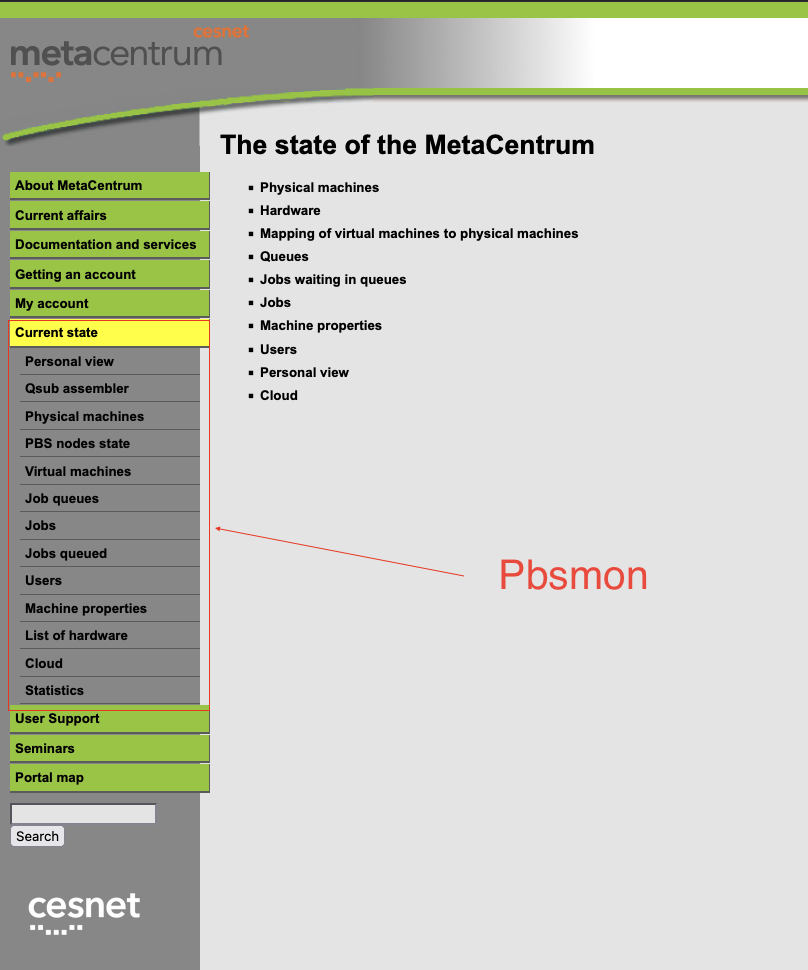
\includegraphics[width=0.5\textwidth]{figures/pbsmon.png}
  \caption{Pbsmon layout}
  \label{fig:pbsmon}
\end{figure}

\newpage
\subsection{Personal view}
\label{subsec:personal-view}
TBD - important, mostly used, ....

\subsection{QSUB assembler}
\label{subsec:qsub-assembler}
TBD - important - 

\subsection{Rest pages}
\label{subsec:rest-pages}
TBD - other pages

\section{Summary of the Analysis}
TBD - Strength and weaknesses


\chapter{Design of the New Solution}
\label{chap:design}

\section{Functional requirements}
\label{sec:functional-requirements}
TBD

\section{GUI design}
\label{sec:gui-design}
TBD - using figma see appendix

\section{Architecture design}
\label{sec:architecture-design}
TBD

\section{Selected technologies}
\label{sec:selected-technologies}
TBD



\chapter{Implementation}
\label{chap:implementation}

\section{System Architecture}
\label{sec:system-architecture-new}

TBD

\section{API}
\label{sec:data-collection-mechanism}

TBD

\subsection{Documentation}
TBD - realized using OpenAPI, automatically generated from code, see appendix

\section{Page views}
\label{sec:page-views}

TBD


\chapter{Testing and Evaluation}

\section{Unit tests}
\label{sec:unit-tests}
TBD

\section{Integration tests}
\label{sec:integration-tests}
TBD

\section{Performance tests}
\label{sec:performance-tests}
TBD


\chapter{Deployment}
TBD

\chapter{Future improvements}


\chapter*{Conclusion}
\addcontentsline{toc}{chapter}{Conclusion}


\appendix
\chapter{OpenStack Response Example}
\label{app:openstack-response-example}

This appendix contains an example of the JSON response structure for the OpenStack cluster named "glados" that is collected by the PBSmon system.

\begin{lstlisting}[caption={Example response for OpenStack cluster "glados"},
  label={lst:openstack-glados-response}]
[
    {
        "CPUs": "40",
        "Hypervisor": "ics-gladosag-007-ostack.priv.cloud.muni.cz",
        "VMs": [
            {
                "CPUs": "38",
                "created": "2020-10-09T09:32:42Z",
                "instance_state": "ACTIVE",
                "name": "RationAI-node-2",
                "user_id": "1633180b677608f61e96784ee5cbc608c0f4b62d@einfra.cesnet.cz"
            }
        ]
    },
    {
        "CPUs": "40",
        "Hypervisor": "ics-gladosag-006-ostack.priv.cloud.muni.cz",
        "VMs": []
    },
    {
        "CPUs": "40",
        "Hypervisor": "ics-gladosag-003-ostack.priv.cloud.muni.cz",
        "VMs": [
            {
                "CPUs": "38",
                "created": "2020-01-17T10:29:22Z",
                "instance_state": "ACTIVE",
                "name": "RationAI-node-1",
                "user_id": "1633180b677608f61e96784ee5cbc608c0f4b62d@einfra.cesnet.cz"
            }
        ]
    },
    {
        "CPUs": "40",
        "Hypervisor": "ics-gladosag-004-ostack.priv.cloud.muni.cz",
        "VMs": []
    },
    {
        "CPUs": "40",
        "Hypervisor": "ics-gladosag-001-ostack.priv.cloud.muni.cz",
        "VMs": [
            {
                "CPUs": "16",
                "created": "2022-08-17T13:07:15Z",
                "instance_state": "ACTIVE",
                "name": "front-82e95edc-1e2d-11ed-9687-0ee20d64cb6e",
                "user_id": "9cd61d48508661633e261f711634b749fdc5d9fcc20769e55baac46ef01c5a63@egi.eu"
            }
        ]
    }
]
\end{lstlisting}

\end{document}
